% == Document Class
%\documentclass{article}
\documentclass[12pt]{article}
\usepackage{lscape}
% == spacing
\usepackage{setspace}
\usepackage{ifdraft}
\usepackage{multirow}
% \doublespacing
% \onehalfspacing
% \singlespacing
\usepackage{listings}
\lstset{breaklines=true} 
\lstset{basicstyle=\small\ttfamily}
\lstset{framesep=4pt}
% == margins
 %% narrow margins (JASA format)
 \addtolength{\hoffset}{-0.75in} \addtolength{\voffset}{-0.75in}
 \addtolength{\textwidth}{1.5in} \addtolength{\textheight}{1.5in}

% medium narrow margins
%\addtolength{\textwidth}{1in} \addtolength{\textheight}{1in}
%\addtolength{\oddsidemargin}{-0.5in} \addtolength{\topmargin}{-0.5in}
%\addtolength{\evensidemargin}{-0.5in}

% == BibTeX packages
\usepackage[longnamesfirst]{natbib}

%
\usepackage{pdflscape}
% == hyperref options
\usepackage{color}
\usepackage[pdftex, colorlinks=false]{hyperref}
\hypersetup{hidelinks}
% == Other Packages
%\usepackage{amsmath, amsmaths, amssymb, url, bm}
\usepackage{amsmath, amssymb, url, bm}
\urlstyle{tt}
\usepackage{rotating}
\usepackage{latexsym}
\usepackage{graphicx}
\usepackage{fancyvrb}  % Verbatim environment
\usepackage{caption}
\usepackage{subcaption}

% == Fonts
% \usepackage{times}
% \usepackage[T1]{fontenc}
% \usepackage{inconsolata}

% == New Commands
% = For general typesetting
\newcommand\spacingset[1]{\renewcommand{\baselinestretch}{#1}\small\normalsize}
\renewcommand\r{\right}
\renewcommand\l{\left}

% = For bibtex
\def\citepos#1{\citeauthor{#1}'s (\citeyear{#1})}
\newcommand\citea{\citeauthor}

% = For general math
\newtheorem{theorem}{Theorem}[section]
\newtheorem{lemma}[theorem]{Lemma}
\newtheorem{corollary}[theorem]{Corollary}
\newtheorem{proposition}{Proposition}
\newtheorem{assumption}{Assumption}
\newcommand{\qed}{\nobreak \ifvmode \relax \else
      \ifdim\lastskip<1.5em \hskip-\lastskip
      \hskip1.5em plus0em minus0.5em \fi \nobreak
      \vrule height0.75em width0.5em depth0.25em\fi}
\DeclareMathOperator*\argmax{argmax}
\DeclareMathOperator*\argmin{argmin}

% = For stats & econometrics
\renewcommand{\epsilon}{\varepsilon}
\newcommand\ud{\mathrm{d}}
\newcommand\dist{\buildrel\rm d\over\sim}
\newcommand\ind{\stackrel{\rm indep.}{\sim}}
\newcommand\iid{\stackrel{\rm i.i.d.}{\sim}}
\newcommand\logit{{\rm logit}}
\newcommand\cA{\mathcal{A}}
\newcommand\E{\mathbb{E}}
\newcommand\V{\mathbb{V}}
\newcommand\cJ{\mathcal{J}}
\newcommand\y{{\bm y}}
\newcommand\X{{\bm X}}
\newcommand\x{{\bm x}}
\newcommand\eps{{\bm\varepsilon}}
\newcommand\zero{{\bm 0}}
\newcommand\one{{\bm 1}}
\newcommand\be{{\bm\beta}}
\renewcommand\b{{\bm b}}
\newcommand\C{{\bm C}}
\newcommand\D{{\bm D}}
\newcommand\I{{\bm I}}
\newcommand\Z{{\bm Z}}
\newcommand\eeta{{\bm \eta}}
\newcommand\bT{{\bm T}}
\newcommand\bt{{\bm t}}
\newcommand\hatT{\hat{T}}
\newcommand\chT{\check{T}}
\DeclareMathOperator*\plim{plim}
\DeclareMathOperator\rank{rank}
\newcommand\indep{\protect\mathpalette{\protect\independenT}{\perp}}
\DeclareMathOperator{\sgn}{sgn}
\def\independenT#1#2{\mathrel{\rlap{$#1#2$}\mkern2mu{#1#2}}}

%%%%%%%%%%%%%%%%%%%%%%%%%%%%%%%%%%%%%%%%%%%%%%%%%%%%%%%%%%%%%%%%%%%%%%%%%%%%%%%%
% == document begins here
%%%%%%%%%%%%%%%%%%%%%%%%%%%%%%%%%%%%%%%%%%%%%%%%%%%%%%%%%%%%%%%%%%%%%%%%%%%%%%%%
\begin{document}

%%%%%%%%%%%%%%%%%%%%%%%%%%%%%%%%%%%%%%%%%%%%%%%%%%%%%%%%%%%%%%%%%%%%%%%%%%%%%%%%
% == Title Page
%%%%%%%%%%%%%%%%%%%%%%%%%%%%%%%%%%%%%%%%%%%%%%%%%%%%%%%%%%%%%%%%%%%%%%%%%%%%%%%%

\newcommand{\blind}{0}

\newcommand{\tit}{Conjoint Survey Design Tool: Software Manual\thanks{Designed as a companion to Hainmueller, Jens, Daniel J. Hopkins, and Teppei Yamamoto. "Causal inference in conjoint analysis: Understanding multidimensional choices via stated preference experiments." Political Analysis 22, no. 1 (2014): 1-30}}

\if0\blind
\title{\bf \tit}
  \author{Anton Strezhnev, Jens Hainmueller, Daniel J. Hopkins, Teppei Yamamoto\\\\Version 3.0}

\date{January 10, 2022}
\maketitle
\if1\blind
\maketitle
\fi

\pdfbookmark[1]{Title Page}{Title Page}

\thispagestyle{empty}
\setcounter{page}{0}
\spacingset{1}

\clearpage

%%%%%%%%%%%%%%%%%%%%%%%%%%%%%%%%%%%%%%%%%%%%%%%%%%%%%%%%%%%%%%%%%%%%%%%%%%%%%%%%
% == Body
%%%%%%%%%%%%%%%%%%%%%%%%%%%%%%%%%%%%%%%%%%%%%%%%%%%%%%%%%%%%%%%%%%%%%%%%%%%%%%%%


\spacingset{1.5}

%%% Section %%%%%%%%%%%%%%%%%%%%%%%%%%%%%%%%%%%%%%%%%%%%%%%%%%%%%%%%%%%%%%%%%%%%
\tableofcontents
\clearpage
\section{Introduction}

The Conjoint Survey Design Tool assists researchers in creating multi-dimensional choice experiments that can be readily incorporated into any pre-existing survey software (such as \href{http://www.qualtrics.com/}{Qualtrics}). Conjoint analysis is a type of survey experiment often used by market researchers to measure consumer preferences over a variety of product attributes. \cite{hainmueller2013} demonstrate the value of this design for political science applications. Conjoint experiments present respondents with a choice among set of profiles composed of multiple randomly assigned attributes. This approach permits researchers to estimate the effect of each individual component on the probability that the respondent will prefer a profile. This software tool is designed as a companion to \cite{hainmueller2013} and provides a graphical user interface for generating conjoint experiments.

\section{A Brief Overview of Conjoint Analysis}

Conjoint survey experiments are made up of a set of  \textbf{choice tasks} or \textbf{trials} performed by the respondent. Each \textbf{task} presents the respondent with a number of \textbf{profiles} and the respondent selects their most preferred alternative. \textbf{Profiles} are comprise of some number of \textbf{attributes} corresponding to particular characteristics of the profiles. Profiles might be candidates for office and attributes could include age, education, and prior experience (as in the choice experiment described by \cite{hainmueller2013}). Each \textbf{attribute} can take on one of a set of discrete and pre-defined \textbf{levels}. For example, an ``age" attribute might have the levels ``young," ``middle-aged," and ``old." In each profile, a level is randomly selected for each attribute from the set of possible levels. \cite{hainmueller2013} show that under this randomization, along with a simple set of consistency assumptions, the average marginal effect of each level is non-parametrically identified. Most importantly, the respondents need not be shown every potential combination of profiles/attributes to identify these component-specific effects. The conjoint experiment thus allows researchers to efficiently run multiple-treatment choice experiments without needing a sample size large enough to present respondents with every possible comparison. For a more detailed explanation of the design, see \cite{hainmueller2013}.

\section{Installation}

There are two ways to run the Conjoint Survey Design Tool (SDT). 

\subsection{Windows Binary}

For Windows users, an executable binary is available for download. This is a self-contained package that requires no additional libraries to function. To use the SDT, download the \texttt{conjointSDT.exe} file to the desired location and run the executable.

A sample survey file, \texttt{immigrant\_demo.sdt}, is included in the Demos folder. 

\subsection{Source Package}
Mac OSX and Linux users do not have standalone executables and need to use the Python source files. Windows users with a Python installation can also use the source package. This, in fact, is advisable as the binary package is much larger than the source since it includes the necessary Python libraries and interpreter. 

The Conjoint SDT is written for Python 3 and requires Python 3.6 or greater. To obtain the most recent release of Python 3, visit \href{https://www.python.org/downloads/}{https://www.python.org/downloads/} 

Mac OSX users should make sure that they have the most recent version of the TCL/TK library installed. If you installed Python. Consult \href{https://www.python.org/download/mac/tcltk/}{https://www.python.org/download/mac/tcltk/} for more information.

To run the Conjoint SDT from Python source, download the \texttt{conjointSDT.py} to the desired directory and run the file through the Python interpreter (this can be done through the command line by calling \texttt{python conjointSDT.py}).

A sample survey file, \texttt{immigrant\_demo.sdt}, is included in the Demos folder.
  

\section{Using the SDT}

\subsection{Main Window}

The main window consists of two panels. The right panel displays the list of attributes in the design. The left panel displays the list of levels that correspond to a chosen attribute. By default, the program opens a blank file with no attributes and levels.

Above the panels are two action menus. The \texttt{File} menu contains the following commands

\begin{figure}[ht!]
\centering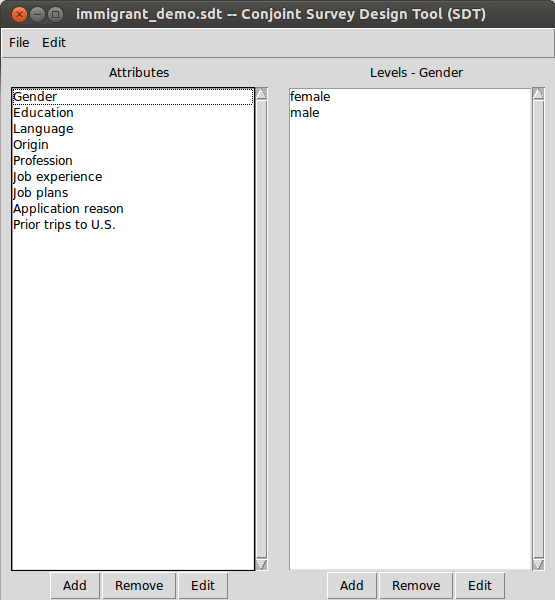
\includegraphics[scale=.6]{graphics/main_window.png}
\caption{Main Window}
\end{figure}

\begin{itemize}
\item \texttt{New}: Begins a new design project. Prompts the user to save any existing work.
\item \texttt{Open}: Opens an existing project. Project filenames all must end in sdt. Note that files with these extensions will not automatically open when clicked on in a file browser.
\item \texttt{Save}: Saves current project. Project filenames must end in .sdt.
\item \texttt{Save As}: Saves current project to a new file.
\item \texttt{Import from CSV}: Imports a set of pre-defined attributes and levels from a Comma Separated Values file. CSV files must contain one line per attribute. The first element of each line defines the name of the attribute. The subsequent elements are the names of the corresponding levels.
\end{itemize}

The \texttt{Edit} menu contains the following commands
\begin{itemize}
\item \texttt{Settings}: Opens the settings menu (see Section 4.2 for details).
\item \texttt{Restrictions}: Opens the profile restrictions menu. Here you can set the attribute/level pairs that should be prevented from appearing in profiles (see Section 4.3 for details).
\item \texttt{Randomization Weights}: Opens the randomization weights menu. Here you can set the probability that each level will be chosen in a randomly generated profile (see Section 4.4 for details).
\item \texttt{Attribute Order Constraints}: Opens the attribute order constraint menu. One option in the Settings menu is to randomize the order of the attributes in the profiles for each respondent. This helps minimize the influence of possible ordering effects. In this panel, you may set constraints on this randomization such that particular sets of attributes are always grouped together in the same block.
\item \texttt{Export to JavaScript}: Exports the current design to a .js file that carries out task and profile generation for each respondent. This file can be integrated directly into Qualtrics. See Section 5 for details.
\item \texttt{Export to .php}: Exports the current design to a .php file that carries out task and profile generation for each respondent. This file can be uploaded to a webserver and queried by your survey software. See Section 6 for details.
\item \texttt{Create Qualtrics Question Templates}: Generates HTML question templates for Qualtrics that have the correct embedded data identifiers for each attribute and level.
\item \texttt{Export design to R}: Exports the design (level probabilities and randomization constraints) to be used by the R package \texttt{cjoint}. 
\end{itemize}

The \texttt{About} menu contains the following command
\begin{itemize}
\item \texttt{License}: View the GPL 3 license information.
\end{itemize}

Below the panels are the Add/Remove/Edit buttons for attributes and levels. To add an attribute to the design or a level to the current active attribute, use the corresponding Add button. To remove an attribute or level, select it in the panel and press the corresponding Remove button. To edit an attribute or level name, select it in the panel and press Edit.



\subsection{Settings}

The settings window contains options related to the .php output file. \textbf{Note:} These settings, aside from the number of tasks and profiles per task are \textit{not} saved as part of the \texttt{.sdt} file.

\begin{figure}[ht!]
\centering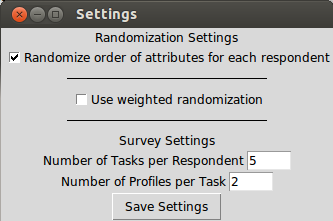
\includegraphics[scale=.6]{graphics/settings_screen.png}
\caption{Settings Window}
\end{figure}

\begin{itemize}
\item \texttt{Randomize order of attributes for each respondent}: Turns on/off attribute order randomization in the .php file output. Select if you want the order in which attributes are presented in a conjoint profile to vary for each respondent. Default True.
\item \texttt{Use weighted randomization}: Enables weighted randomization of levels. Select if you have defined non-uniform randomization weights and want the randomization script to use them. Default False.
\item \texttt{Prevent identical profiles}: Ensures that no task can have two profiles that have exactly the same levels for all attributes. With sufficiently many attributes/levels, the chances of getting a task with identical profiles is already very low and the presence of cross-profile restrictions creates additional complications for interpreting the AMCE estimand. Default False.
\item \texttt{Number of Tasks per Respondent}: Sets the number of tasks assigned to a single respondent. Default 5
\item \texttt{Number of Profiles per Task}: Sets the number of profiles presented in a single task. Default 2.
\end{itemize}

\subsection{Profile Restrictions}

This panel allows you to restrict the appearance of certain attribute/level combinations in profiles presented to respondents. By default, every possible level combination has the possibility of being shown to a respondent. For some designs, certain combinations may be nonsensical, impossible or confusing to respondents. You may want to prohibit these combinations from being displayed in profiles. For example, in the immigration conjoint experiment in \cite{hainmueller2013}, profiles could not indicate that the prospective immigrant did not have at least a college education and worked in a high-skill occupation (e.g. research scientist, computer programmer). These combinations were a priori excluded because of their implausibility.

\begin{figure}[ht!]
\centering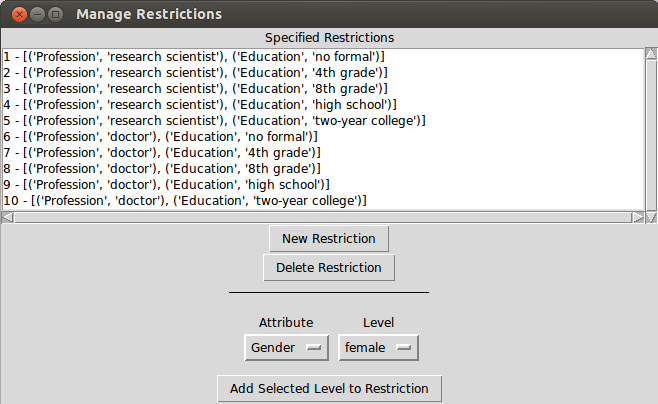
\includegraphics[scale=.6]{graphics/restriction_screen.png}
\caption{Profile Restrictions Window}
\end{figure}

Best practices in the conjoint literature suggest that these types of prohibitions should be used sparingly as they represent deviations from a fully randomized design. As \cite{Orme2002} notes 
\begin{quote} 
``Too many prohibitions, in the best case, can lead to imprecise utility estimation and, in the worst case, confounded effects and the complete inability to calculate stable utilities."
\end{quote}

In this screen, restrictions are specified individually. Each restriction represents a unique combination of attribute-levels that are prohibited from being displayed. Note, that if three or more levels are specified in a restriction, only the combination of \emph{all} of those levels is prevented from being displayed. For example, if a restriction prevents a profile from containing attribute-levels 1-A, 2-B and 3-C, absent additional restrictions, the profile could still contain 1-A, 2-B and 3-D or 1-E, 2-B, and 3-C.   

To create a new restriction, click on \texttt{New Restriction}. To delete an existing restriction, click on that restriction in the panel and then press \texttt{Delete Restriction}. To add a particular level to a restriction, select that restriction in the panel, choose your desired attribute and level from the drop-down menus and click \texttt{Add Selected Level to Restriction}.

\textbf{Note}: In the current version of the Conjoint SDT, restrictions must be deleted manually. If a particular attribute or level is subsequently removed in the main panel, it is not automatically removed from any previously specified restrictions.

\subsection{Weighted Randomization}

By default, each attribute level has an equal probability of being drawn. That is, for a given attribute, each defined level has the same probability of appearing in a profile. However, you may want to define a non-uniform randomization scheme such that some levels are more likely to appear in a profile than others. 

\begin{figure}[ht!]
\centering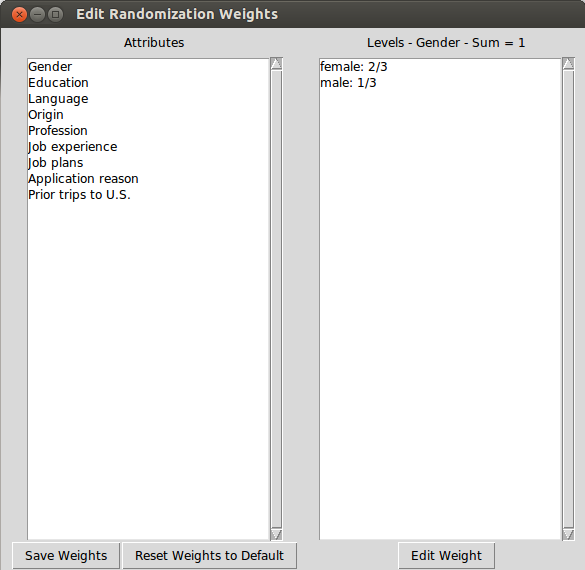
\includegraphics[scale=.6]{graphics/weight_screen.png}
\caption{Weighted Randomization Window}
\end{figure}

This window allows you to assign selection probabilities for each level within an attribute. By default, each level within an attribute has an equal probability of selection into the profile. To change a weight, select a level from the panel and click \texttt{Edit Weight}. Standard probability constraints apply. Probabilities must be between $0$ and $1$ and must sum to $1$ across all levels within an attribute. The sum across weights within an attribute is displayed above the levels panel. To save the weights, click \texttt{Save Weights}. To reset the weights to the default uniform randomization scheme, click \texttt{Reset Weights to Default}.

\textbf{Warning}: In order for these weights to be properly exported to the randomization scripts, you also need to make sure to check the \texttt{Use Weighted Randomization} option in the \textbf{Settings} menu. This setting is \textbf{not saved} when you save the \text{.sdt} file, so be sure to enable it before using \texttt{Export to PHP}.

\textbf{Note}: If attributes and levels are subsequently added to the design, the weighted probabilities will reset to the default (uniform randomization). It is recommended that you define all of the attributes and levels that you wish to include in your design and then alter the randomization weights. 

\subsection{Attribute Order Constraints}

If you choose to randomize the order in which attributes are displayed for each respondent, you may still want to keep some attributes in a pre-defined order to ease comprehension and improve readability. For example, you may want to group thematically related attributes together.

\begin{figure}[ht!]
\centering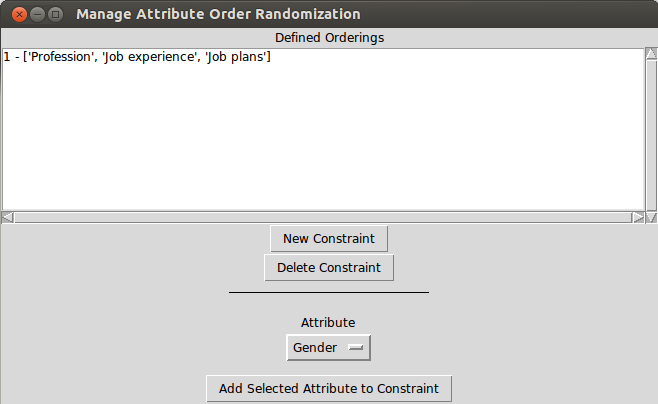
\includegraphics[scale=.6]{graphics/order_screen.png}
\caption{Attribute Order Constraint Window}
\end{figure}

This window allows you to define blocks of attributes that will always be presented to respondents in the same order. To create a new block click \texttt{New Constraint}. To delete an existing block click \texttt{Delete Constraint}. To add an attribute to a constraint, select the constraint from the panel, choose an attribute from the drop-down menu and press \texttt{Add Selected Attribute to Constraint}. The order of the attributes within the block will match the constraint list. So in the above figure, the ``Profession" attribute will always be followed by the ``Job experience" and ``Job plans" attributes (in that order). 

Note that if you define multiple blocks, only the attributes \textit{within} each block will be ordered. The blocks themselves are \textit{not} constrained such that block one always follows block two.

\textbf{Note}: As with the profile restrictions, if you choose to delete an attribute you will have to manually remove any corresponding order randomization constraint 

\section{Export to JavaScript}

To incorporate your conjoint design into Qualtrics, you can generate a snippet of javascript code that will randomly generate a full set of tasks for a respondent according to your specified settings. The snippet can be added to the custom javascript of any survey question that appears prior to your conjoint question block (typically the survey consent page if you have one).

The script will assign embedded data fields in Qualtrics for each randomized attribute and level. These fields all have the following structure: 

\texttt{F-[task number]-[attribute number]} matches the attribute name corresponding to Task \texttt{[task number]}, Attribute \texttt{[attribute number]}. \texttt{F-[task number]-[profile number]-[attribute number]} matches the selected level corresponding to Task \texttt{[task number]}, Profile \texttt{[profile number]}, Attribute \texttt{[attribute number]}. For example, the embedded data field \texttt{F-1-3-2} will contain the level corresponding to Task 1, Profile 3, Attribute 2. Likewise, the embedded data field \texttt{F-3-3} will contain the attribute name corresponding to Task 3, Attribute 3.

\subsection{How to embed your design into a Qualtrics question}

If you are using the Qualtrics survey software, it is very easy to integrate the .js file you have exported with your survey flow. The following instructions will walk you through the process of incorporating your conjoint design into a Qualtrics question.
\begin{enumerate}
\item Select the first question in your survey (i.e. the consent page) (Really, any question that appears on a page prior to the conjoint block should work.)
\item Open the question's custom JavaScript (this appears under Edit Question - Question Behavior - JavaScript).
\item Copy the source code from your generated .js file below the commented line \texttt{/*Place your JavaScript here to run when the page loads*/} (this is inside the  \texttt{addOnload} function). The code snippet will update the embedded data fields assigned to the respondent when the respondent loads the page.
\item If you have already created the question designs within Qualtrics, you can pipe the embedded data fields into any question element within the survey. \footnote{For more information on piping text from embedded data fields, see \href{http://www.qualtrics.com/university/researchsuite/basic-building/editing-questions/piped-text/}{http://www.qualtrics.com/university/researchsuite/basic-building/editing-questions/piped-text/}.} 
\item If you have not created the questions, a basic set of templates for the conjoint tasks can be generated using the \texttt{Create Qualtrics Question Templates} command in the \texttt{Edit} menu. This command will create an .html file for every task in your design.
\item To add a question to your design, create a new item in your Qualtrics survey and select the ``Multiple Choice" item type. Edit the question in HTML view, open the source code from one of the .html files in a text editor (such as Notepad), and copy the source into the HTML view. Repeat for each task.
\item You may then edit the question text, labels and responses to match your design. Note that references to the embedded data fields have the format \texttt{\$\{e://Field/F-[TASK]-[ATTRIBUTE]\}} (for attribute names) and \texttt{\$\{e://Field/F-[TASK]-[ATTRIBUTE]-[PROFILE]\}} (for attribute levels)
\end{enumerate}

In addition to pasting in the JavaScript code, you will also need to manually initialize each embedded data field in the Survey Flow in order for Qualtrics to correctly export these fields to the results CSV. To do this

\begin{enumerate}
\item In your Qualtrics control panel, navigate to the Survey Flow.
\item Add a new ``Embedded Data" element to the top of your survey flow. Make sure that this element is above your conjoint question blocks \textbf{and above to the question that contains the JavaScript snippet} in the survey flow.
\item Add a unique field for each attribute and each level embedded data field in your survey (e.g. F-1-1, F-2-1, F-1-3-2). The total number of fields will depend on the number of tasks, profiles and attributes. You can consult the generated HTML Question Templates (see above) for a list of all attribute and level identifiers used in your survey. You may leave the assigned value in this element to ``Value will be set from Panel or URL" as it will be subsequently modified by the JS code.
\end{enumerate}

Note that if you skip this step and field the survey without initializing the fields in the Survey Flow, the questions do seem to correctly appear and the assigned attributes and levels for each respondent \textit{are} saved but will not be part of the CSV export. If you are having trouble getting the assigned attributes and levels to appear in your exported CSV results and you have already fielded your survey, make sure you add the embedded data field to your Survey Flow as above and re-export the CSV.

If you can come up with a faster way of doing this, please let me know! Unfortunately, Qualtrics appears to need all exported embedded data fields to be defined in the Survey Flow.

\section{Export to PHP}


\textcolor{red}{\large This approach is no longer recommended. It is much easier to use the ``Export to JavaScript" approach to embed the randomization script within a Qualtrics survey as this does not require using a second external server.}

To incorporate your conjoint design into an online survey experiment, you can export it to a .php file. When queried, the .php script will generate a set of tasks for a single respondent according to the settings that you have specified. The script will return an array object with the following key-value structure:

\texttt{F-[task number]-[attribute number]} matches the attribute name corresponding to Task \texttt{[task number]}, Attribute \texttt{[attribute number]}. \texttt{F-[task number]-[profile number]-[attribute number]} matches the selected level corresponding to Task \texttt{[task number]}, Profile \texttt{[profile number]}, Attribute \texttt{[attribute number]}. For example, the key \texttt{F-1-3-2} matches the level corresponding to Task 1, Profile 3, Attribute 2. Likewise, the key \texttt{F-3-3} returns the attribute name corresponding to Task 3, Attribute 3.

Below is a sample array (two tasks per respondent, two profiles per task, nine attributes) from the immigration conjoint experiment included in the Demos folder.

\begin{lstlisting}
{"F-1-1":"Origin","F-1-1-1":"Mexico","F-1-2":"Language","F-1-1-2":"fluent English","F-1-3":"Profession","F-1-1-3":"nurse","F-1-4":"Job experience","F-1-1-4":"3-5 years","F-1-5":"Job plans","F-1-1-5":"no plans to look for work","F-1-6":"Gender","F-1-1-6":"female","F-1-7":"Application reason","F-1-1-7":"seek better job","F-1-8":"Education","F-1-1-8":"8th grade","F-1-9":"Prior trips to U.S.","F-1-1-9":"many times as tourist","F-1-2-1":"Sudan","F-1-2-2":"fluent English","F-1-2-3":"computer programmer","F-1-2-4":"5+ years","F-1-2-5":"interviews with employer","F-1-2-6":"male","F-1-2-7":"seek better job","F-1-2-8":"high school","F-1-2-9":"many times as tourist","F-2-1":"Origin","F-2-1-1":"Iraq","F-2-2":"Language","F-2-1-2":"fluent English","F-2-3":"Profession","F-2-1-3":"financial analyst","F-2-4":"Job experience","F-2-1-4":"5+ years","F-2-5":"Job plans","F-2-1-5":"will look for work","F-2-6":"Gender","F-2-1-6":"female","F-2-7":"Application reason","F-2-1-7":"reunite with family","F-2-8":"Education","F-2-1-8":"4th grade","F-2-9":"Prior trips to U.S.","F-2-1-9":"six months with family","F-2-2-1":"Iraq","F-2-2-2":"broken English","F-2-2-3":"janitor","F-2-2-4":"1-2 years","F-2-2-5":"no plans to look for work","F-2-2-6":"male","F-2-2-7":"escape persecution","F-2-2-8":"4th grade","F-2-2-9":"six months with family"}
\end{lstlisting}

This output can then be fed dynamically into your online survey.

\subsection{How to embed your design into a Qualtrics question}

If you are using the Qualtrics survey software, it is very easy to integrate the .php file you have exported with your survey flow. The following instructions will walk you through the process of incorporating your conjoint design into a Qualtrics question.
\begin{enumerate}
\item Upload the .php file to a web server (make sure that the web server has support for PHP version 5.2 or greater). If you \textbf{absolutely} must use an older version of PHP, you will need to modify the .php file to support a \texttt{json\_encode()} function. A number of possible implementations are available by searching online. 
\item In your Qualtrics control panel, navigate to the Survey Flow.
\item Add a new ``Web Service" element to the top of your survey flow.\footnote{For more information on how to create a Web Service element, see \href{https://www.qualtrics.com/support/survey-platform/survey-module/survey-flow/advanced-elements/web-service/}{https://www.qualtrics.com/support/survey-platform/survey-module/survey-flow/advanced-elements/web-service/}.} Make sure that this element is above your question blocks in the survey flow.
\item In the URL field, enter the address of your .php file, set the method to GET, and press ``Test URL."  
\item If the URL is set correctly, a pop-up window should appear containing a list of fields corresponding to your attributes. Select all of the fields (click on ``all" in the upper-left corner) and click ``Add Embedded Data"
\item The attribute fields should now appear in the web service panel below ``Set Embedded Data"
\item If you have already created the question designs within Qualtrics, you can pipe the embedded data fields into any question element within the survey. \footnote{For more information on piping text from embedded data fields, see \href{http://www.qualtrics.com/university/researchsuite/basic-building/editing-questions/piped-text/}{http://www.qualtrics.com/university/researchsuite/basic-building/editing-questions/piped-text/}.} 
\item If you have not created the questions, a basic set of templates for the conjoint tasks can be generated using the \texttt{Create Qualtrics Question Templates} command in the \texttt{Edit} menu. This command will create an .html file for every task in your design.
\item To add a question to your design, create a new item in your Qualtrics survey and select the ``Multiple Choice" item type. Edit the question in HTML view, open the source code from one of the .html files in a text editor (such as Notepad), and copy the source into the HTML view. Repeat for each task.
\item You may then edit the question text, labels and responses to match your design. Note that references to the embedded data fields have the format \texttt{\$\{e://Field/F-[TASK]-[ATTRIBUTE]\}} (for attribute names) and \texttt{\$\{e://Field/F-[TASK]-[ATTRIBUTE]-[PROFILE]\}} (for attribute levels)

\end{enumerate}

\section{Export to R}

If you would like to use the design tool to specify a conjoint design for use in the \texttt{cjoint} package, use the ``Export Design to R'' menu option. This will ask you to save a \texttt{.dat} file which will contain the design's attributes, levels and level assignment probabilities. 

This file can be passed to the \texttt{makeDesign()} function in the \texttt{cjoint} R package. Please consult the documentation for the \texttt{cjoint} R package located on CRAN for more information on where to pass the design file and for general instruction on how to perform the analysis.

\section{Contact}

If you have further questions about using the Conjoint SDT or wish to report a bug, please do not hesitate to contact Anton Strezhnev at \href{mailto:astrezhnev@uchicago.edu}{astrezhnev@uchicago.edu}.

\section{License}

This program is free software: you can redistribute it and/or modify it under the terms of the GNU General Public License as published by the Free Software Foundation, either version 3 of the License, or (at your option) any later version.

This program is distributed in the hope that it will be useful, but WITHOUT ANY WARRANTY; without even the implied warranty of MERCHANTABILITY or FITNESS FOR A PARTICULAR PURPOSE. See the GNU General Public License for more details.

You should have received a copy of the GNU General Public License along with this program.  If not, see $\langle$\href{http://www.gnu.org/licenses/}{http://www.gnu.org/licenses/}$\rangle$.


\clearpage
\bibliographystyle{chicagoa}
\bibliography{conjointsdtbib}

\end{document}
%%%%%%%%%%%%%%%%%%%%%%%%%%%%%%%%%%%%%%%%%%%%%%%%%%%%%%%%%%%%%%%%%%%%%%%%%%%%%%%%
% == document ends here
%%%%%%%%%%%%%%%%%%%%%%%%%%%%%%%%%%%%%%%%%%%%%%%%%%%%%%%%%%%%%%%%%%%%%%%%%%%%%%%%
